\documentclass{amsart}
\usepackage[margin=1.2in]{geometry}
\usepackage{fancyhdr}
\usepackage{graphicx,hyperref,xcolor} 
\usepackage{todonotes}
% Set up the fancy header and footer
\pagestyle{fancy}
\fancyhead{}  % Clear all headers and footers
\fancyfoot[C]{\thepage} 

\hypersetup{
    colorlinks=true,
    linkcolor=blue,
    filecolor=magenta,      
    urlcolor=cyan,
    pdftitle={DD-MED},
    pdfpagemode=FullScreen,
    }

\title{CA STV Modeling}
\author{Matthew Jones, Hane Lee, Jay Lee, Max Springer with support from Christopher Donnay, Moon Duchin, and Peter Rock.}
\date{\today}


\begin{document}

\maketitle

%%% other sections about 12 pages

\section{How it works}
Single transferable vote, or STV, is a ranked-choice voting system that can be used to elect 
one or more seats.\footnote{In the case of electing a single seat, STV is often called 
instant-runoff voting (IRV).} In STV, a threshold of first-place votes is required to be elected.
If no candidate meets the threshold, the candidate with the fewest first-place votes is eliminated,
and their votes are transferred to the next candidate on those ballots.
This is repeated until a candidate reaches the threshold; the candidate is elected, and
their votes in surplus of the threshold are transferred to the next candidate on those ballots.
This is repeated until all seats have been filled.

Here is a simple example of how STV works. \todo{Add example}

In our example above, there were a few algorithmic decisions that had to be made. 
The first is the threshold. 
Above we used the \emph{Droop quota}, the most common threshold used in STV elections.
Let $m$ denote the number of seats to be filled ($m$ stands for \emph{magnitude}).
The Droop quota is calculated as
\[\left\lfloor\frac{\text{\# of votes}}{m+1} + 1\right\rfloor,\]
where $\lfloor \cdot \rfloor$ denotes rounding down to the nearest integer.
One way to interpret the Droop quota is that it is the minimum number of votes such 
that no more than $m$ candidates can achieve the quota.
There are other thresholds that can be used, including some which updated dynamically
as the tabulation process progresses.\todo{Cite}
For the remainder of this report, we will use the Droop quota.

Another important decision is the method for transferring votes. 
One option is called \emph{fractional transfer}. In fractional transfer, once a candidate is elected,
any ballot with that candidate in first place is discounted by a factor of 
\[\frac{\text{\# of votes}- \text{threshold}}{\text{\# of votes}},\]
and the vote transfers to the next candidate on the ballot.
This is how we transferred votes in our example above.
In Cambridge, Massachusetts, they use a method called \emph{random transfer}.\todo{Cite}
In random transfer, once a candidate is elected, they randomly select 
\[\text{\# of votes}- \text{threshold}\]
ballots to keep, and the votes are transferred to the next candidate on those ballots.
The unselected ballots are no longer used in the tabulation process.

There are other transfer methods? including \todo{cite} 

Finally, there are two edge cases that need to be handled.
The first is the method for handling  multiple candidates 
crossing the threshold in a single round. Either elect all of them in that round,
or elect the one with the most votes, and proceed to another round of tabulation.
This decision affects the order in which candidates are elected and which can even 
alter the winner set.
The second consideration is a method for handling ties. Ties can occur whenever two or more
candidates have the same number of first-place votes.\todo{Cite, https://www.portland.gov/sites/default/files/2024/Portland-District-1-Certified-Abstract-Nov-2024.pdf}\footnote{This is not an edge case; ties occur 
in real-world STV elections. See Round 8 in District 1 of the Portland, OR city council election in 2024.}
One method is to just randomly select one of the tied candidates; another is to use the 
first-place vote count from the first round of tabulation.  

Taken together, these algorithmic decisions make up an STV election.






\section{Background and prior use}


\subsection{History in the United States}
%% jay more detail/citations
Despite sparse implementation today, STV has a long and storied history in the United States.
Starting in the early 20th century, multi-seat STV was adopted for use in local elections across some two dozen cities,
including New York, NY; Cincinnati, OH; Cambridge, MA; and Sacramento, CA. Almost all of them eventually repealed STV;
Cambridge is the notable exception, having used STV continuously since 1941 to elect
its nine city council members. \todo{Cite, https://www.cambridgema.gov/Departments/electioncommission/cambridgemunicipalelections}
See Figure \ref{fig:stv_timeline_US} for a timeline of STV's history in the United States.

The story of STV's adoption and repeal in Cincinnati is emblematic of both the success of this reform strategy, 
and of the societal friction it created. Like many cities in the United States at the turn of the 20th century, 
Cincinnati city hall was a partisan machine; here controlled by the Republicans. 
The chair of the Hamilton County Republican Committee Bob Cox once said, ``The people do the voting. 
I simply see that the right candidates are elected."
In the 1921 election, Republicans won 31 out of 32 seats on the city council, despite Democrats
making up about 44\% of the electorate.

In response, reformers from the Charter Committee introduced an STV reform measure to the 1924 ballot,
which passed with 69\% of the vote. By most measures, the reform was a success. 
The city elected its first Black councillors, with 10 out of 15 councils elected under STV having
at least one Black councillor.
However, the success of Black candidates caused intense friction with White citizens of Cincinnati.
Starting in the mid-1930s, a wave of repeal measures were intoduced.
After the possibility arose that the council would elect a Black mayor, the fifth repeal 
effort passed in 1957, with White-majority precincts voting for repeal 2-1 and Black-majority 
precincts voting 4-1 to keep STV. \todo{Cite}

The story in New York is largely the same, with Tammany Hall's Democratic machine controlling a 
supermajority of the Board of Aldermen despite only being supported by a modest majority of voters. 
The implementation of STV in 1937 led 
to a wave of women, people of color, and minority parties winning seats on the new City Council. 
When two communists were elected in the 1940s, the energy from the Red Scare proved too much and 
STV was repealed in 1947. The two major political parties also led the charge for repeal in New York 
and other cities, as shifting coalitions sought to increase their influence over legislatures and voters. 
\todo{Cite, https://fairvote.org/wp-content/uploads/2024/03/Proportional-Representation-in-NYC.pdf}

What is illustrated in the history of STV in the United States is that the reform worked as intended.
STV, through multi-winner elections and voting thresholds, enabled candidates without majority support 
to be elected and gave political voice to marginalized groups, and (along with other Progressive-era government 
reforms) it helped break entrenched urban political machines. Ultimately, this success was its own downfall.

In the 21st century, we see a renewed interest in STV, with cities like New York, NY adopting single-seat STV 
for primary elections; Portland, OR and Portland, ME adopting multi-seat STV for city council; and 
San Francisco and Oakland, CA adopting single-seat STV for municipal elections. Voters in three states 
(or state equivalents) have approved single-seat STV for state elections: Maine in 2016, Alaska in 2020, 
and the District of Columbia in 2024.

\begin{figure}
    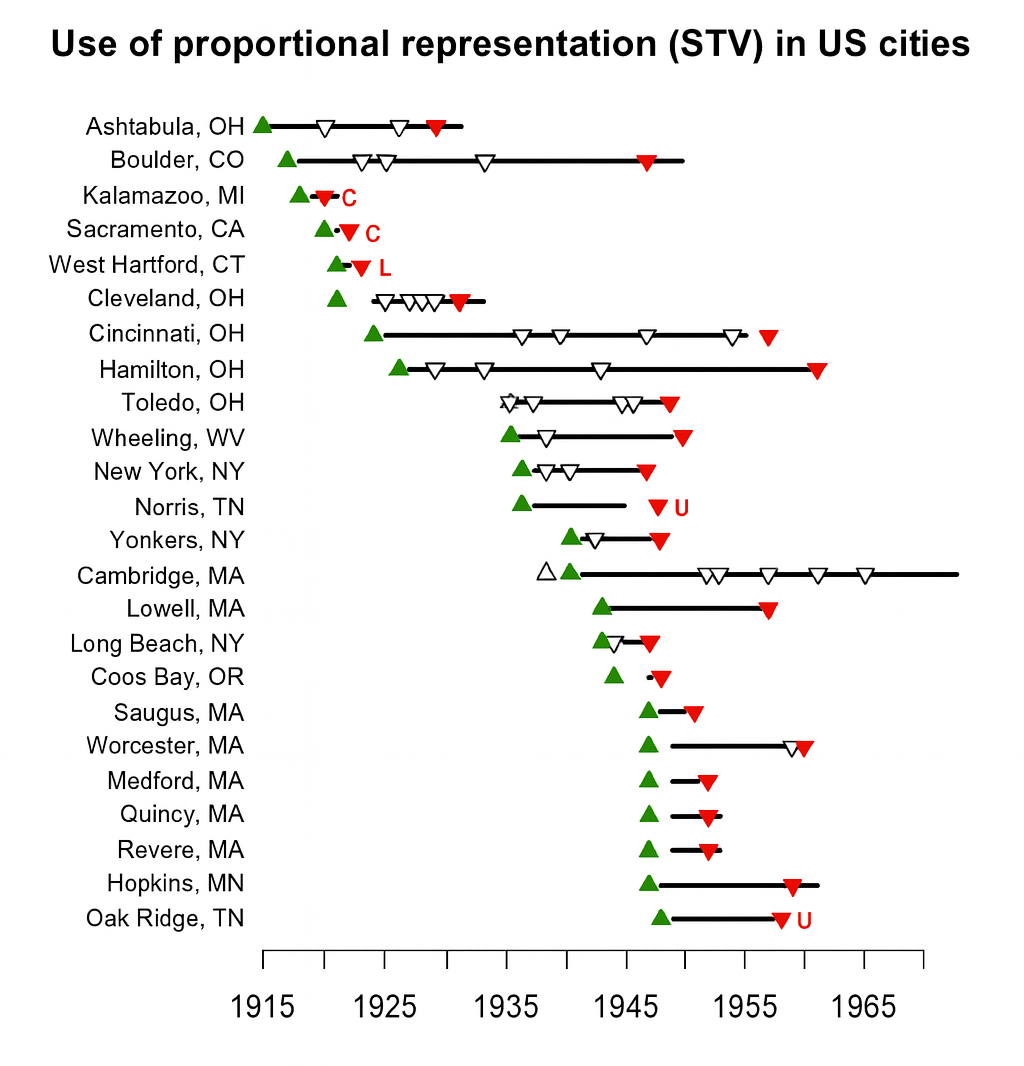
\includegraphics[width=0.5\textwidth]{figures/stv_timeline_us.png}
    \caption{A timeline of STV's history in the United States.
    Upward green triangles denote adoption of STV, while downward red triangles denote repeal of STV.
    White triangles denote a failed attempt. Figure source:
    https://www.voteguy.com/2016/12/30/pr-graphic-for-public-use/}
    \label{fig:stv_timeline_US}
\end{figure}



\subsection{Use in other countries}

 %% jay 

STV has been used for upwards of a century around the world (most widely in the Anglosphere) to elect national, 
regional, and local governments. Global uses include:

\begin{itemize}
    \item \textbf{Australia} uses STV to elect both chambers of its Federal Parliament, one or both chambers in the parliaments of 
        its states and internal territories, and certain local councils across the country. The Australian Senate uses multi-seat STV 
        and staggered terms
        to elect 12 members representing each state and 4 members from the territories, and the House of 
        Representatives uses single-seat STV to elect members from single-member districts covering the entire country.
        \todo{Cite, https://www.ecanz.gov.au/electoral-systems}
    \item \textbf{Ireland} uses multi-seat STV to elect its D\'ail (lower house of parliament), delegates to the 
        European Parliament, and every local council in the country; and single-seat STV to elect the President. 
        Members of the D\'ail are chosen in 43 multi-member districts electing between three and five members each. 
        \todo{Cite, https://www.electoralcommission.ie/general-elections/}
    \item \textbf{New Zealand} allows for multi-seat STV to elect local councils, and it is currently used by 
        15 local authorities for their elections. \todo{Cite, https://www.stv.govt.nz/index.shtml}
    \item The \textbf{United Kingdom} uses multi-seat STV in two of its constituent countries. Northern 
        Ireland uses multi-seat STV to elect its Assembly, with 18 districts each electing five members. Both 
        Northern Ireland and Scotland use multi-seat STV to elect every local council. 
        \todo{Cite, https://electoral-reform.org.uk/where-is-single-transferable-vote-used-in-the-uk/}
\end{itemize}

\section{Pros and Cons}
\subsection{Pros}
\begin{itemize}
    \item[\bf{Flexible:}] STV can be used with or without districts. It is flexible enough to be used 
                    either to elect a single winner per district, to elect multiple winners per district,
                    or to elect all winners at large. This flexibility allows STV to be used in a variety of contexts,
                    from at-large city councils to districted legislative bodies.

    \item[\bf{Proportional tendencies:}] STV in the multi-winner setting tends to produce more
                    proportional outcomes than plurality voting. This is in part because STV dampens the 
                    power of ballots that have already had a candidate elected, thus giving smaller
                    voting blocs the change to elect a candidate of choice.

    \item[\bf{Non-partisan:}] Unlike some list-based voting systems, STV does not require 
                        candidates to run under a party label. This lowers the barrier to entry
                        for candidates who may not enjoy the support of a political party.
    \item[\bf{Local alignment:}] STV is already used in six California cities to elect one or more winners, 
                        with another city currently implementing the system for future use.\todo{Cite, https://fairvote.org/our-reforms/ranked-choice-voting-information/?section=jurisdictions-using-rcv} 
                        Voters in two of the state's most populous cities are already familiar with the system, 
                        and local election officials in some large counties have previously piloted voter education 
                        and implemented STV.
\end{itemize}

\subsection{Cons}

%%% flip of  non-partisan, vote leakage 
\begin{itemize}
    \item[\bf{Complex mechanism:}] STV is a relatively complex voting mechanism, and it can be difficult 
                    for voters to understand how their vote is converted into an outcome. %% more info required from voter

    \item[\bf{Voter burden:}] As a voting system, STV \emph{technically} requires that each voter provides 
                    a complete ballot. That is, each ballot needs to list a candidate in each ranking position.
                    This can be a burden for voters, especially if they are not familiar with the candidates
                    or if they are voting in an election with a long ballot. %% if you want your vote to fully "count"

    \item[\bf{Vote exhaustion:}] If a voter does not complete their ballot, it is possible that 
                    through candidate elimination their vote will no longer be an active 
                    part of the tabulation process. 

    \item[\bf{Vote leakage:}] Votes ``for" a party can leak to other parties.
\end{itemize}

In practice, much of the cons list can be mitigated through voter education and outreach. 
The mechnism can be explained, and voters can be encouraged to complete their ballots.
Cities that have implemented STV have found that mistakes on ballots decrease over time
as voters become more familiar with the system. \todo{Cite}




CA Single-subject rule concerns

\section{Modeling STV in CA}

We consider shifting California's lower and upper legislative chambers to STV.
There are 80 districts in the lower chamber and 40 districts in the upper chamber.
We compare electing 5 members per district with STV to 4 members per district with STV, 
as well as the current system of single member districts with plurality voting.  
We identify two different axes to evaluate the impact of the reform along: racial 
representation and partisan representation.
For racial representation we consider splitting the electorate into Hispanic and non-Hispanic voters.
For partisan representation we consider splitting the electorate into Democratic and Republican voters.

%%% not meant to be complete but illustrative

In order to evaluate the impact of shifting to STV, we need to generate realistic ranked-choice ballots for voters.

\subsection{Generating realistic ranked preferences for voters}
One of the primary challenges with deciding on an electoral reform is that there is not a wealth of 
historical ranked-choice data available to construct realistic preferences for voters, thus making
it difficult to evaluate the impact of the reform. There is a growing body of work in 
computational social choice that allows us to generate realistic preferences for voters 
using parameterized mathematical models. 

While a full discussion of the mathematical models is beyond the scope of this report, we briefly introduce them here. 
We use three different models to generate ranked-ballots 
for voters: the slate-Plackett-Luce sampler, the slate-Bradley-Terry sampler, and the Cambridge sampler.
We first assume that voters are divided into two blocs and each bloc has a corresponding slate of candidates.
Each bloc of voters has an underlying preference for their slate of candidates over the other slate.
Each bloc also has preference for the candidates within their own slate.
To create a ballot for a voter, a model first decides the order in which the slates appear on the ballot.
Then, for each slate, the model decides the order in which the candidates appear, and fills them 
in on the ballot in that order.

Consider the following example.\todo{Add example}

%% describe impulsive, deliberative, cambridge 
%% shorthand descriptions

\subsection{Evaluating the impact of the reform}
\todo[inline]{Story of the results goes here.}

\section{Conclusion}
\todo[inline]{Conclusion goes here.}
\end{document}